% !TEX root = ../../main.tex
\chapter{Statistical Analysis}
\label{ch:stats}

In this chapter, the quantitative strategy used to compare the recorded data to SM predictions, and to set limits on BSM theoretical models, is outlined. The invariant mass distribution, $m(\ell\nu J)$, is used as a discriminant in this search, with an optimized binning strategy as detailed in~\Sect{\ref{ch:stats:vb}}. In \Sect{\ref{ch:stats:ml}}, a maximum-likelihood (ML) fit of the data to a background-only hypothesis, to determine the normalizations of the \Wjets and \ttbar backgrounds, is described. The systematic uncertainties described in~\Ch{\ref{ch:syst}} are included in the fit as nuisance parameters (NP), and the SRs and CRs are fit simultaneously. In \Sect{\ref{ch:stats:ul}}, a test statistic based on the profiled log likelihood ratio, used to create upper limits on production cross sections, is outlined. 

%
\section{Variable Binning}
\label{ch:stats:vb}
In the ML fit (\Sect{\ref{ch:stats:ml}}), the $m(\ell\nu J)$ distribution is binned. In order to optimize the number of bins, and the width of each bin, simulated signal samples are used to find the mass resolution of the signal model as a function of signal mass.  For each mass point, the $m(\ell\nu J)$ distribution is fit with a Breit-Wigner function\footnote{
	Although using a model with a Breit-Wigner convolved with a Gaussian would extract a width close to the simulated width, the approximate experimental resolution of the width is of interest for determining the binning.
}. The mean and width are extracted from the fit, where the width is used as an estimate of the signal mass resolution. In~\Fig{\ref{fig:sig_fit}}, an HVT $Z'$ signal model at $m=2\,\TeV$ is used to illustrate the fit and extraction of the mass resolution. In~\Tab{\ref{tab:resns}}, the natural resonance width and the extracted resonance width are provided for the HVT $Z'$ and RS $G^*$ signal models. In~\Fig{\ref{fig:binning}}, a linear fit is used to parameterize the extracted mass resolutions for both signal models.  For the HVT $Z'$ (RS $G^{*}$) model, the natural width is approximately 3\,\% (6\,\%) the resonance mass, while the extracted resolution is approximately 5\,\% (9\,\%) the resonance mass, indicating detector effects inflate the natural resonance width by approximately 2-3\,\%. 

\begin{wrapfigure}{r}{.5\textwidth}
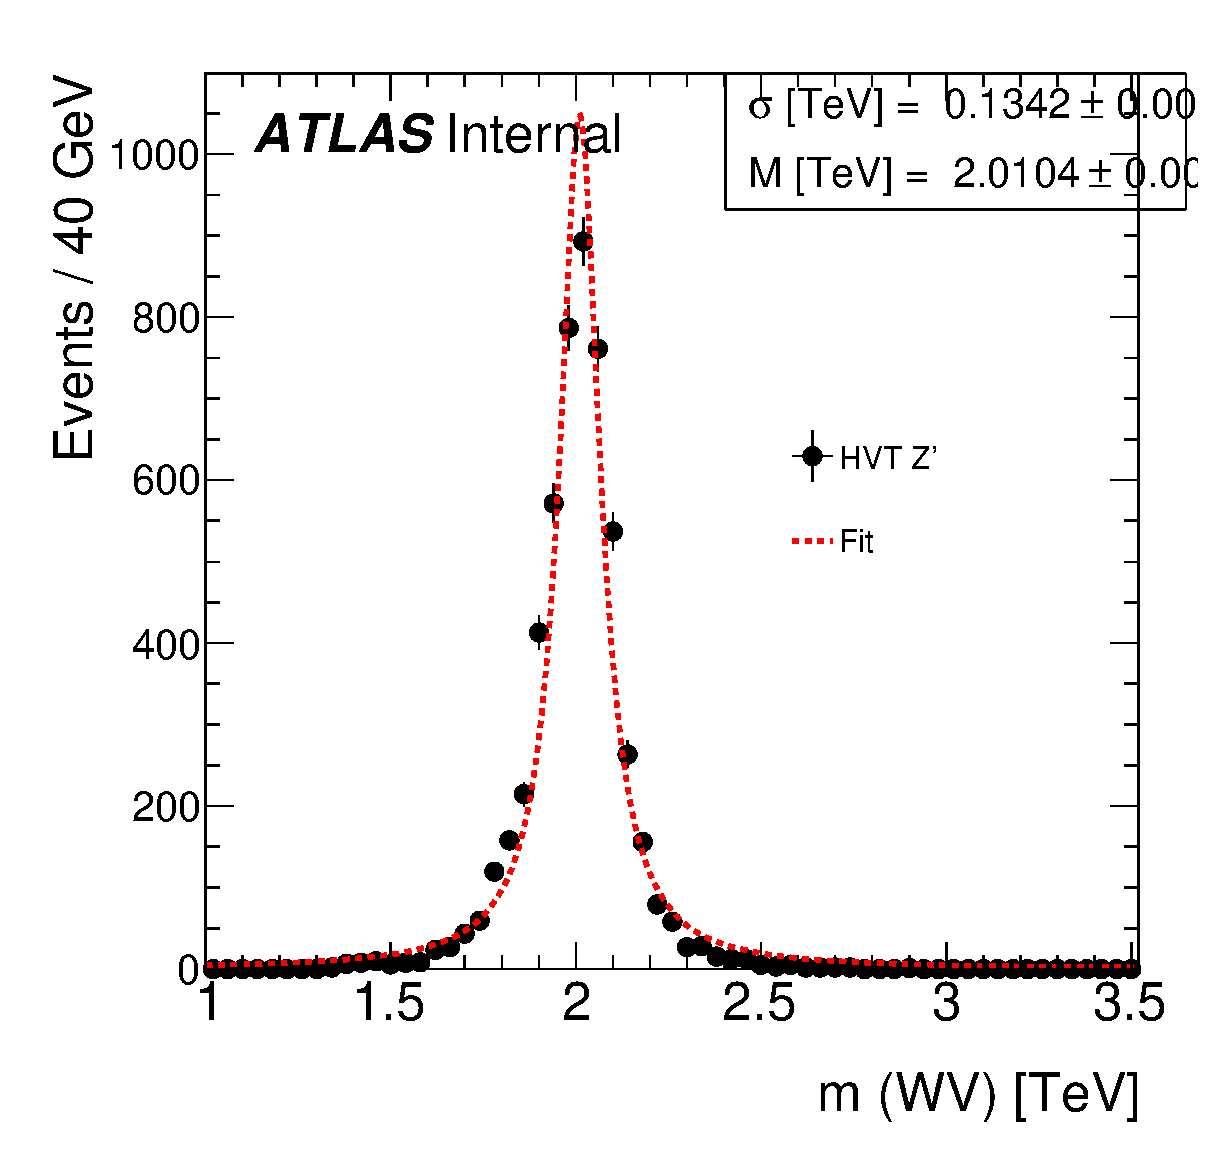
\includegraphics[width=.99\linewidth]{figures/StatisticalAnalysis/fit_HVT_WW_15}
\caption[Extraction of signal mass resolution]{An HVT $Z'$ signal sample at $m=2\,\TeV$\,is fit with a Breit-Wigner function to extract the width, $\Gamma$, and estimate the signal mass resolution.}
\label{fig:sig_fit}
\end{wrapfigure}

The final binning is optimized using the HVT $Z'$ 
signal model with ggF selection. This search uses 500\,\GeV\, as the lowest bin edge, adding bins with a width at least as large as the resolution determined from the extracted linear fit. In the high mass region, there are low background statistics. To avoid bins with too few entries, in this region bin widths are enlarged such that the ratio of the statistical uncertainty to the background expectation in a bin is below a threshold. The final binning for the ggF selection includes 20 bins, with all overflows included in the last bin. For the VBF selection, background statistics decrease much more rapidly, and only 11 bins are used. The first nine bins are identical to the ggF selection, while the final two bins are enlarged to address the decreasing background statistics. 

\begin{table}[htb]
\centering
\begin{tabular}{c|c|c|c|c}
\hline\hline
Signal Mass [\TeV] & \multicolumn{2}{c|}{HVT $Z'$} & \multicolumn{2}{c}{RSG $G^{*}$} \\\cline{2-5}
& $\Gamma_{\rm exp.}$ [\GeV] & $\Gamma_{\rm meas.}$ [\GeV]& $\Gamma_{\rm exp.}$ [\GeV] & $\Gamma_{\rm meas.}$ [\GeV]\\\hline
0.8 & 32 & 74 & 46 & 90 \\
1.6 & 51 & 113 & 96 & 149 \\
2.4 & 74 & 153 & 148 & 238 \\\hline\hline
\end{tabular}
\caption[Expected and measured resonance widths]{Theoretical and measured resonance widths for HVT $Z'$ (model-B, $g_v=3$) and RS $G^{*}$ ($k/\overline{M}_{\rm Pl}=1.0$) signal models. The natural width for the HVT $Z'$ (RS $G^{*}$) signal model is approximately 3\,\% (6\,\%) the mass of the resonance, while experimental effects inflate the resolution by approximately 2\,\% (3\,\%).}
\label{tab:resns}
\end{table}



\begin{figure}[htb]
\centering
%\subfloat[]{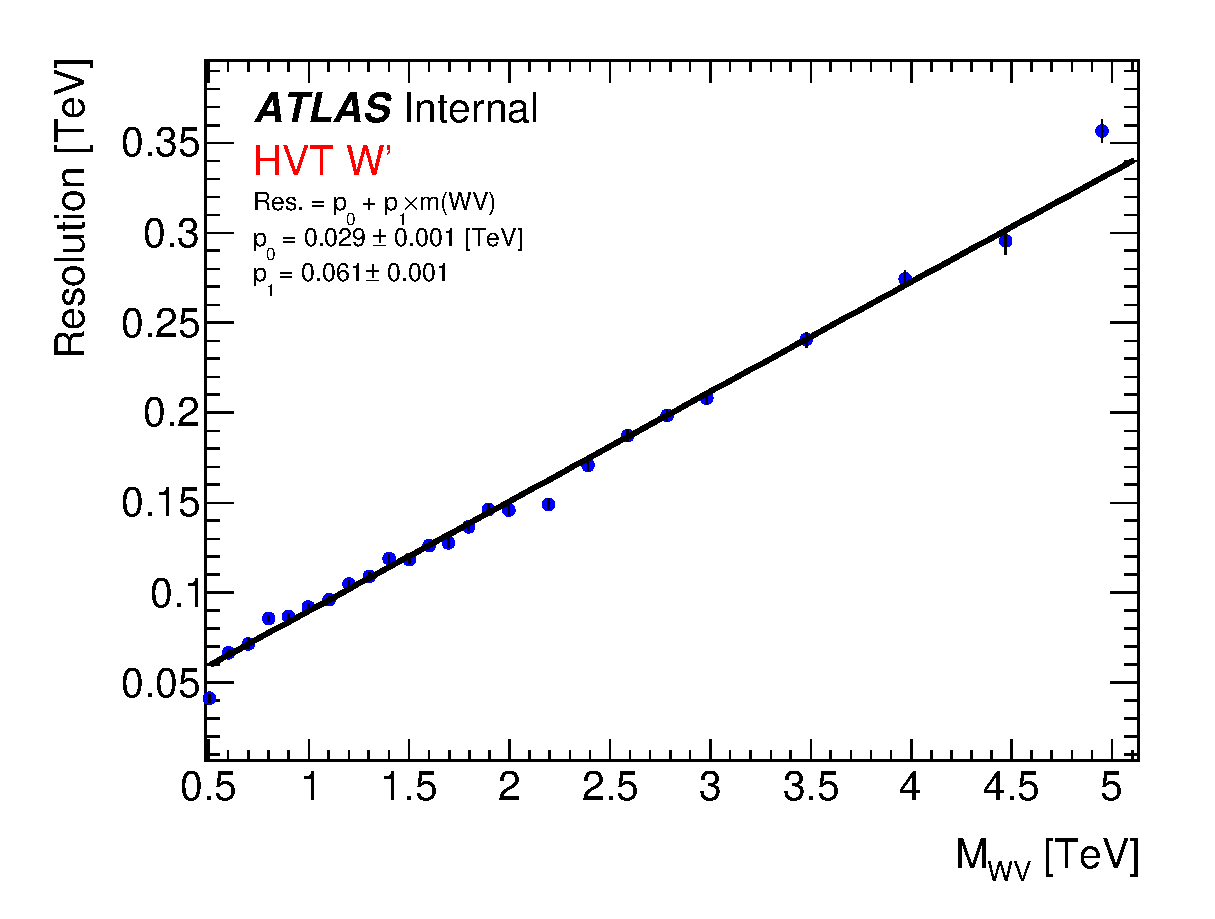
\includegraphics[width=.49\textwidth]{figures/StatisticalAnalysis/HVT_WZ}\label{fig:binning:a}}
\subfloat[]{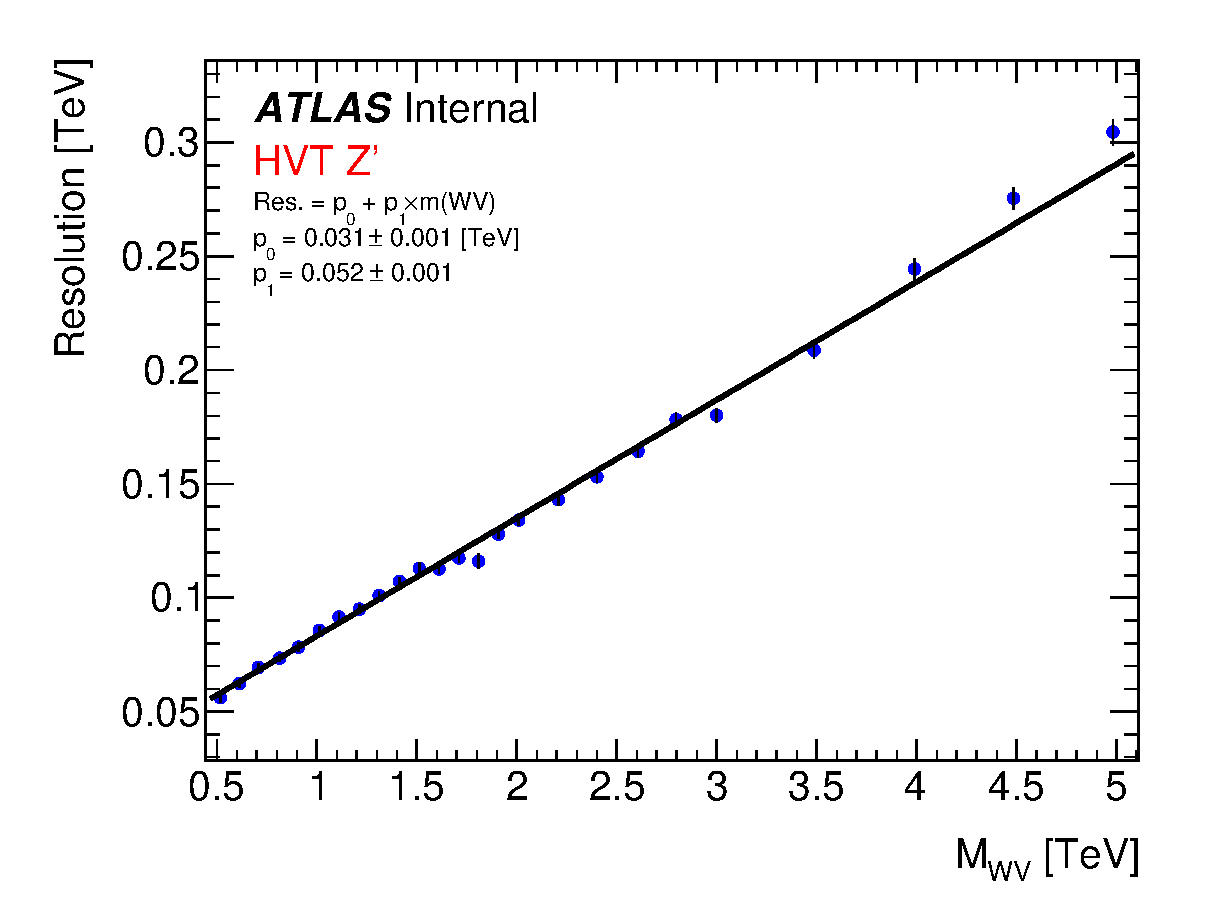
\includegraphics[width=.49\textwidth]{figures/StatisticalAnalysis/HVT_WW}\label{fig:binning:b}} %\\
\subfloat[]{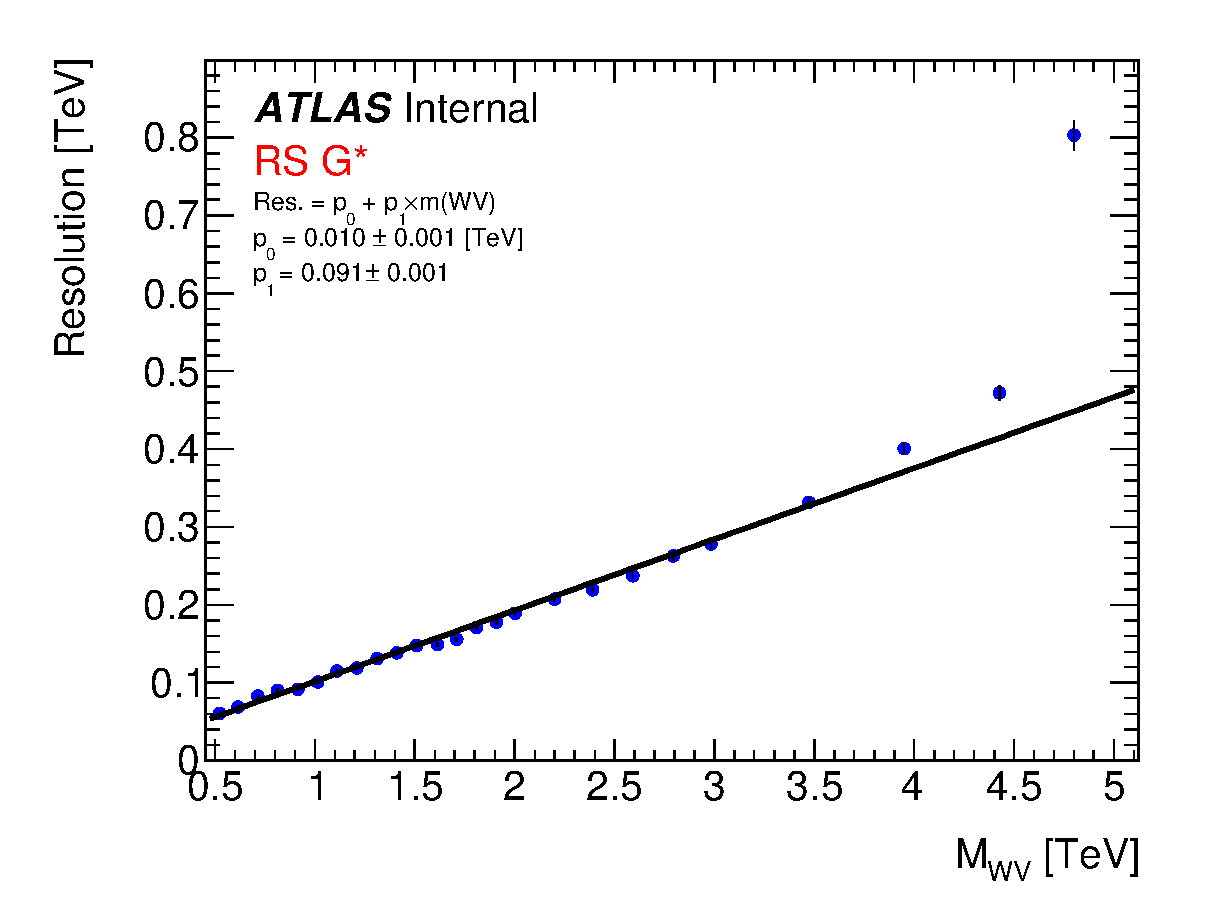
\includegraphics[width=.49\textwidth]{figures/StatisticalAnalysis/RS_G_WW}\label{fig:binning:c}}
\caption[Resolution of simulated signal samples]{Mass resolution of simulated signal samples as a function of $m(WV)$ for %\protect\subref{fig:binning:a} HVT $W'$, 
\protect\subref{fig:binning:b} HVT $Z'$ and \protect\subref{fig:binning:c} RS $G^*$ signal models. The fit to the HVT $Z'$ signal model was used to determine the binning in this analysis.} 
\label{fig:binning}
\end{figure}



%
\section{Binned Maximum Likelihood Fit}
\label{ch:stats:ml}
A simultaneous binned ML fit~\cite{lh_stats} of the $m(\ell\nu J)$ distribution in the SRs and CRs is performed on the MC prediction to the recorded data. Due to their large overlap, the $WW$ and $WZ$ channels are analyzed separately. Additionally, the VBF and ggF selections are fit separately. Signal models with ggF (or qqF) production are analyzed with the fit to the ggF selection, while signal models with VBF production are analyzed with the fit to the VBF selection. A summary of which of the four fits is considered for each benchmark signal model is given in~\Tab{\ref{tab:sig_fits}}. For each fit, there is a common normalization factor for the HP and LP regions, for each of the two main backgrounds ($\Wjets$ and $\ttbar$). These normalizations are free to float in the fit and constrained by the dedicated CRs.

\begin{table}[b!]
\bigskip
\centering
\resizebox{\textwidth}{!}{%
\begin{tabular}{l|cc|cc}
\hline\hline
Model&\multicolumn{2}{c|}{ggF Selection (SRs \& CRs)}&\multicolumn{2}{c}{VBF Selection (SRs \& CRs)}\\\cline{2-5}
&$WW$&$WZ$&$WW$&$WZ$\\\hline
\textbf{Scalar Heavy Higgs}&&&&\\
\,\hfill ggF prod.&\checkmark&&&\\
\,\hfill VBF prod.&&&\checkmark&\\\hline
\textbf{HVT} $\mathbf{Z'}$&&&&\\
\,\hfill qqF prod.&\checkmark&&&\\
\,\hfill VBF prod.&&&\checkmark&\\\hline
\textbf{HVT} $\mathbf {W'}$&&&&\\
\,\hfill qqF prod.&&\checkmark&&\\
\,\hfill VBF prod.&&&&\checkmark\\\hline
\textbf{RS} $\mathbf{G^{*}}$&\checkmark&&&\\\hline\hline
\end{tabular}
}
\caption[Selection regions used in the simultaneous maximum likelihood fit for the benchmark signal models]{Summary of the selection regions included in the maximum likelihood fit for each benchmark signal model. For each selection, all of the corresponding high purity (HP) and low purity (LP) signal regions (SR) and control regions (CR) are included. For example, in the fit corresponding to the ggF selection, $WW$ channel, the following regions are included in the simultaneous fit: HP SR ($WW$), LP SR ($WW$), HP \Wjets CR, LP \Wjets CR, HP \ttbar CR and LP \ttbar CR, with all regions passing the ggF selection.}
\label{tab:sig_fits}
\end{table}

The likelihood function is a product of the Poisson distributions for each selection region and bin included in the fit. The Poisson distribution for observing a number of events, $n_{\rm obs}$, with an expected number of events, $n_{\rm exp}$, is given in~\Eqn{\ref{eq:pois_prob}}. Systematic uncertainties are included as constrained NPs in the fit with Gaussian, or log-normal distributions. 
The histograms for the backgrounds are based on MC samples with finite statistics. The Barlow-Beeston ``lite'' method~\cite{bin_stats} is used to account for bin-by-bin statistical uncertainties by adding a NP for each bin in each region. These NPs represent the statistical uncertainty in a bin from each background, added in quadrature.
The normalizations for the minor backgrounds are included as NPs in the fit, with Gaussian constraints on the production cross section of 11\,\%, 11\,\%, and 30\,\% for the \Zjets, \Singlet, and SM diboson backgrounds, respectively, according to SM measurements. The full likelihood function is expressed in~\Eqn{\ref{eq:lh_func}}.
\begin{eqnarray}
P(n_{\rm obs}|n_{\rm exp}) &=& \frac{\left(n_{\rm exp}\right)^{n_{\rm obs}}e^{-n_{\rm exp}}}{n_{\rm obs}!} \label{eq:pois_prob}\\
L(\mu,\bm{\theta})&=&\prod_{j\in\{\rm SRs,\, CRs\}}\prod_{i\in\{\rm bins\}} P(N_{ij}|\mu s_{ij}+ B_{ij})\prod_{l\in\{\rm NPs\}}{\rm Nuis}(\theta_l) \label{eq:lh_func} \\
B_{ij}&=&\mu_{\ttbar} b_{ij}^{\ttbar} + \mu_{\Wjets}b_{ij}^{\Wjets}+ b_{ij}^{\rm other} \label{eq:bkg_exp}
\end{eqnarray}
The signal strength, $\mu$, parameterizes the production of signal events, where $\mu=1$ corresponds to the nominal signal hypothesis and $\mu=0$ corresponds to the background-only hypothesis.  The parameter $\bm{\theta}$ represents the collection of all NPs. In the likelihood function, the index $j$ runs over the SRs and CRs in the fit, the index $i$ runs over the bins of the $m(\ell\nu J)$ distribution in each region, and the index $l$ runs over all of the NPs considered. In the Poisson distribution functions, for each bin $i$ and region $j$, $N_{ij}$, is the number of observed data events, $s_{ij}$ is the number of expected signal events, and $B_{ij}$ is the number of expected background events. $B_{ij}$ is defined in~\Eqn{\ref{eq:bkg_exp}}, where $\mu_{\ttbar}$ ($\mu_{\Wjets}$) is the normalization factor for the \ttbar (\Wjets) background, and $b_{ij}^{x}$ is the expected number of background events for background process $x$ (i.e. \ttbar, \Wjets, or other = \Singlet, \Zjets, and SM dibosons). 

For each systematic uncertainty, ``up'' and ``down'' histograms are generated, corresponding to the variation of the systematic uncertainty by $\pm 1\sigma$. The impact of the systematic uncertainty on the nominal event yield is parameterized by a NP, $\theta$, such that $\theta=\pm1$ corresponds to the variation of the systematic uncertainty by $\pm 1 \sigma$. The event yield is thus factored according to the separate contributions from each NP, as shown in~\Eqns{\ref{eq:syst_imp}}{\ref{eq:delta_np}}, where $(\mu s +B)^{\pm,\,0}$ corresponds to the event yield from the ``up'' ($+$), ``down'' ($-$), or nominal ($0$) variations. The NPs have an applied Gaussian or log-normal constraint, centered at 0 with width 1. This parameterization of the impact of the systematic uncertainty variations is denoted by $\text{Nuis}(\theta_l)$ in~\Eqn{\ref{eq:lh_func}}. For each NP, correlations are taken into account between bins in the final discriminant, between regions in the fit, and between background and signal distributions. 

\begin{eqnarray}
\mu s+B&=&(\mu s+B)^0\prod_l\left(1+\Delta_l\theta_l\right)\label{eq:syst_imp}\\
\Delta_l&=& \begin{cases}\frac{(\mu s+B)^+-(\mu s+B)^0}{(\mu s+B)^0} & \theta_l\geq 0 \\ \frac{(\mu s+B)^0-(\mu s+B)^-}{(\mu s+B)^0} & \theta_l<0  \end{cases} \label{eq:delta_np}
\end{eqnarray}


For some of the systematic uncertainties, their estimated variations were calculated using MC samples with limited statistics. In order to avoid the effects of statistical fluctuations, some of the variations of the systematic uncertainties are smoothed. The event yield in bin $i$ for the ``up'' or ``down'' histogram of a smoothed systematic uncertainty is set according to the prescription in~\Eqns{\ref{eq:smoothing:a}}{\ref{eq:smoothing:b}}.

\begin{eqnarray}
(\mu s+B)^{\pm}_i&=&(\mu s + B)^0_i\left[1+\lambda_i^{\pm}\right] \label{eq:smoothing:a}\\
\lambda_i^{\pm}&=&\frac{1}{4}\left( \left[(\mu s+B)^{\pm}_{i-1}-(\mu s+B)^0_{i-1}\right] +2\left[(\mu s+B)^{\pm}_{i} - (\mu s+B)^0_{i}\right]  \right.\nonumber \\
& & \left.+ \left[(\mu s+B)^{\pm}_{i+1}-(\mu s+B)^0_{i+1}\right]  \right) \label{eq:smoothing:b}
\end{eqnarray}


%
\section{Upper Limits on Cross Section}
\label{ch:stats:ul}
A test statistic, $\tilde{q}_{\mu}$, based on the log of the profile likelihood ratio~\cite{lh_stats}, is used to test values of the signal strength, $\mu$, for each signal model, and set upper limits on the production cross section. The profile likelihood ratio, $\tilde{\lambda}(\mu)$, is defined in~\Eqn{\ref{eq:plr}}, where the signal strength is constrained to be non-negative ($\mu\geq0$) because the contribution to the event yield from a signal model is assumed to be non-negative.

\begin{equation}
\tilde{\lambda}(\mu)=\begin{cases} \frac{L(\mu,\hat{\hat{\bm{\theta}}}(\mu))}{L(\hat{\mu},\hat{\bm{\theta}})}&\hat{\mu}\geq 0 \\ \frac{L(\mu,\hat{\hat{\bm{\theta}}}(\mu))}{L(0,\hat{\hat{\bm{\theta}}}(0))} & \hat{\mu}< 0 \end{cases}
\label{eq:plr}
\end{equation}

In the numerator, $\hat{\hat{\bm{\theta}}}(\mu)$ represents the value of $\bm{\theta}$ that maximizes the likelihood function, $L$, for a fixed value of $\mu$. This is the conditional ML estimator of $\bm{\theta}$, and is a function of $\mu$. The denominator is the ML function; that is, $\hat{\mu}$ and $\hat{\bm{\theta}}$ are the unconditional ML estimators of $\mu$ and $\bm{\theta}$. The value of the estimator, $\hat{\mu}$, that maximizes the likelihood function is allowed to be negative so that it can be modeled by a Gaussian distributed variable. For cases where $\hat{\mu}<0$, the denominator in the profile likelihood ratio is fixed to the physical value that best describes the data, with $\mu=0$ and $\hat{\hat{\bm{\theta}}}(\mu=0)$.

The value of $\tilde{\lambda}$ is constrained by $0\leq\tilde{\lambda}\leq 1$, where values closer to 1 indicate better agreement between the observed data and the hypothesized signal model with signal strength, $\mu$. The test statistic, $\tilde{q}_{\mu}$, is defined in~\Eqn{\ref{eq:qmu}}, where larger values of $\tilde{q}_{\mu}$ indicate less compatibility between the observed data and the hypothesized signal strength. The test statistic is set to zero for $\hat{\mu}>\mu$ because an estimated $\hat{\mu}$ larger than the hypothesized value does not represent lower compatibility with the observed data, and is not part of the region rejected by a one-sided upper limit. 

\begin{equation}
\tilde{q}_{\mu} = \begin{cases}-2\ln\tilde{\lambda}(\mu)&\hat{\mu}\leq \mu\\ 0 & \hat{\mu}>\mu \end{cases} \label{eq:qmu}
\end{equation}

In order to quantify the level of agreement, a $p$-value can be calculated from the test statistic with the probability distribution function (PDF) of the test statistic, $f(\tilde{q}_{\mu}|\mu)$, as shown in~\Eqn{\ref{eq:pmu}}. Asymptotic distributions of $f(\tilde{q}_{\mu}|\mu)$ are taken from~\Ref{\cite{lh_stats}} and used for tested signal mass points below $1.6\,\TeV$\,($1.0\,\TeV$) for fits to regions with ggF (VBF) selection. For higher signal masses, the PDFs are estimated with an ensemble of 50,000 generated pseudo-experiments using toy MC methods. Near the boundary between the two regimes, the asymptotic and pseudo-experiment limits are found to agree well, while in the highest mass region above $4\,\TeV$, a discrepancy of approximately 20-30\,\% is found, with the pseudo-experiment distributions producing more conservative upper limits. 

\begin{equation}
p_{\mu} = \int_{\tilde{q}_{\mu,\,\rm obs}}^{\infty} f(\tilde{q}_{\mu}|\mu) d\tilde{q}_{\mu}  \label{eq:pmu}
\end{equation}
 

A modified frequentist approach, called the $CL_s$ method~\cite{cls_stats}, is employed to set the final upper limits. The $CL_s$ method uses the ratio of two frequentist confidence levels (CL) as shown in~\Eqnrange{\ref{eq:cls:a}}{\ref{eq:cls:d}}.
Values of $CL_{s+b}$ close to zero indicate the signal model is highly disfavored. 
%Values of $CL_b$ close to one indicate the background-only hypothesis is highly disfavored. 
A model with signal strength, $\mu$, is excluded if $CL_s<0.05$, corresponding to a CL of 95\,\%. By scanning values of $\mu$ for a specific model, the 95\,\% CL upper limit is set by finding $\mu^{\rm up}$ such that $CL_s=0.05$. In \Eqn{\ref{eq:cls:c}}, $p_{s+b}$ describes the probability, under the assumption of the signal plus background hypothesis with signal strength $\mu$, of measuring a test statistic, $\tilde{q}_{\mu}$, that is equally or less compatible with the tested signal strength than the observed test statistic, $\tilde{q}_{\mu,\,\rm obs}$.  Likewise,~\Eqn{\ref{eq:cls:d}} describes the probability, under the assumption of the background-only hypothesis, of measuring a value of the test statistic greater than or equal to the value observed. That is, the probability to correctly reject the tested value of $\mu$ when the background-only hypothesis is correct. 

\begin{eqnarray}
CL_s&=&\frac{CL_{s+b}}{CL_b}\label{eq:cls:a} \\
&=&\frac{p_{s+b}}{1-p_b}\label{eq:cls:b}\\
p_{s+b}&=& \int_{\tilde{q}_{\mu,\,\rm obs}}^{\infty} f(\tilde{q}_{\mu}|\mu) d\tilde{q}_{\mu} \label{eq:cls:c}\\
1-p_b&=& \int_{\tilde{q}_{\mu,\,\rm obs}}^{\infty} f(\tilde{q}_{\mu}|\mu=0) d\tilde{q}_{\mu}  \label{eq:cls:d}
\end{eqnarray}

With respect to a true frequentist CL, the $CL_s$ method is conservative~\cite{cls_stats}. The denominator ($1-p_b$) is always less than or equal to one, thus the requirement $CL_s<0.05$ is more stringent than $p_{s+b}<0.05$.  The benefit of the $CL_s$ approach is that the p-value is penalized for regions where the search has no sensitivity. If a search has a small sensitivity to $\mu$ (expected signal yield is small or zero with respect to the background yield), the model will still be rejected with a probability close to 5\,\%. In the $CL_s$ method, the PDFs of the test statistic for the signal model and for the background-only model have a large overlap if the search has a low sensitivity; thus, as $p_{s+b}$ decreases so does $(1-p_b)$, preventing $CL_s<0.05$. 





% HVT WZ
% bins: 500 559 622 689 760 835 915 1000 1090 1185 1286 1393 1507 1628 1756 1892 2036 2189 2351 2523 3593 3841
% bw: 59 63 67 71 75 80 85 90 95 101 107 114 121 128 136 144 153 162 172 1070 248
% No stats
% bins: 500 559 622 689 760 835 915 1000 1090 1185 1286 1393 1507 1628 1756 1892 2036 2189 2351 2523 2706 2900 3106 3324 3556 3802
% bw: 59 63 67 71 75 80 85 90 95 101 107 114 121 128 136 144 153 162 172 183 194 206 218 232 246

% HVTWW
% bins: 500 557 617 680 747 817 891 969 1051 1137 1227 1322 1422 1527 1638 1754 1876 2005 2140 2282 2432 2589
% bw: 57 60 63 67 70 74 78 82 86 90 95 100 105 111 116 122 129 135 142 150 157
% No stats
% bins: 500 557 617 680 747 817 891 969 1051 1137 1227 1322 1422 1527 1638 1754 1876 2005 2140 2282 2432 2589 2755 2967 3152 3347 3552 3768
% bw: 57 60 63 67 70 74 78 82 86 90 95 100 105 111 116 122 129 135 142 150 157 166 212 185 195 205 216

% RSGWW
% bins: 500 556 617 684 757 837 924 1019 1122 1235 1358 1492 1639 1799 1974 2165 2373 2600
% bw: 56 61 67 73 80 87 95 103 113 123 134 147 160 175 191 208 227
% No stats
% bins: 500 556 617 684 757 837 924 1019 1122 1235 1358 1492 1639 1799 1974 2165 2373 2600 2848 3118 3413 3735
% bw: 56 61 67 73 80 87 95 103 113 123 134 147 160 175 191 208 227 248 270 295 322